\documentclass[12pt,a4paper]{article}
\usepackage[utf8]{inputenc} 
\usepackage[T1]{fontenc}		       
\usepackage{lmodern}			       
\usepackage{babel} 
\usepackage{amsmath}
\usepackage{amsfonts}
\usepackage{amssymb}
\usepackage{graphicx}
\usepackage{xcolor}
\usepackage{mathtools}
\usepackage{fancyhdr}
\usepackage{enumitem}
\usepackage{tcolorbox}
\usepackage{stmaryrd}
\usepackage{dsfont}
\usepackage{pgf, tikz}
\usetikzlibrary{shapes.misc}
\usepackage[linesnumbered,ruled,vlined]{algorithm2e}
\usepackage[text={15cm,24.5cm},centering]{geometry}

% Définir le texte affiché en fin de page
\pagestyle{fancy}
\fancyhf{}  % Clear the default headers and footers
\rfoot{\hrule
    \vspace{0.3cm}
    \noindent\textsf{Félix de Brandois}
    \hfill \thepage
}
\renewcommand{\headrulewidth}{0pt}

% Style de l'entete
\newcommand{\entete}{
    \noindent\textbf{INSA - ModIA, 4$^e$ année.}
    \hfill \textbf{Années 2023-2024}
    
    \begin{center}
        \textbf{\LARGE Théorie des graphes - Annale 1}
    \end{center}
}


\begin{document}

\entete

\vspace{0.5cm}

\section*{Exercice 1}

On a 4 villes : $V_1$, $V_2$, $V_3$ et $V_4$. \\
Il existe des vols directs de : $V_1$ vers $V_2$, $V_1$ vers $V_4$, $V_2$ vers $V_3$, $V_3$ vers $V_1$, $V_3$ vers $V_4$ et $V_4$ vers $V_2$. \\

\begin{enumerate}
    \item Montrer qu'il existe au moins un vol avec 2 escales de $V_i$ à $V_j$ pour $i \neq j$.
    \item Ecrire la matrice d'adjacence, et trouver tous les trajets d'une ville à une autre avec 1 escale (utiliser la multiplication latine).
    \item Comment retrouver le résultat de la question 1. avec la multiplication latine ?
\end{enumerate}


\color{blue}

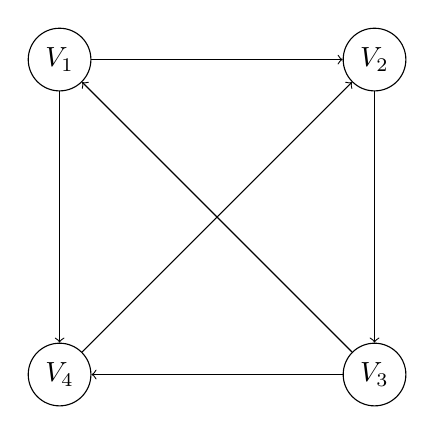
\begin{tikzpicture}
    \node[draw, circle] (V1) at (0,0) {$V_1$};
    \node[draw, circle] (V2) at (4,0) {$V_2$};
    \node[draw, circle] (V3) at (4,-4) {$V_3$};
    \node[draw, circle] (V4) at (0,-4) {$V_4$};
    
    \draw[->] (V1) -- (V2);
    \draw[->] (V1) -- (V4);
    \draw[->] (V2) -- (V3);
    \draw[->] (V3) -- (V1);
    \draw[->] (V3) -- (V4);
    \draw[->] (V4) -- (V2);
\end{tikzpicture}



\begin{enumerate}
    \item Enoncé erroné
    
    \item La matrice d'adjacence est la suivante :
    
    \[
    M = \begin{pmatrix}
    0 & 12 & 0 & 14 \\
    0 & 0 & 23 & 0 \\
    31 & 0 & 0 & 34 \\
    0 & 42 & 0 & 0
    \end{pmatrix}
    \]
    
    On cherche les trajets d'une ville à une autre avec 1 escale. On utilise la multiplication latine. On a :
    
    \[
    M^2 = \begin{pmatrix}
        0 & 142 & 123 & 0 \\
        231 & 0 & 0 & 234 \\
        0 & 312 + 342 & 0 & 314 \\
        0 & 0 & 423 & 0
    \end{pmatrix}
    \]    

    \item On utilise la multiplication latine pour 2 escales :
    \[
        M^3 = \begin{pmatrix}
            x & 0 & 1423 & 1234 \\
            x & x & 0 & 2314 \\
            0 & 3142 & x & 0 \\
            4231 & 0 & x & x
        \end{pmatrix}
        \]
\end{enumerate}

\color{black}

\section*{Exercice 2}
$Q_n$ : Graphe sommets n-uplets de 0 ou 1 adjacents si ils diffèrent seulement de 1 bit. \\

Montrer que $Q_n$ est hamiltonien pour $n \geq 2$.

\color{blue}

$Q_2$ :

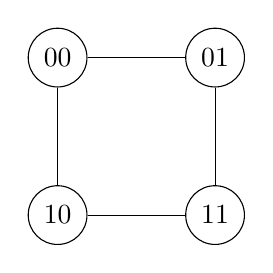
\begin{tikzpicture}
    \node[draw, circle] (00) at (0,0) {00};
    \node[draw, circle] (01) at (2,0) {01};
    \node[draw, circle] (11) at (2,-2) {11};
    \node[draw, circle] (10) at (0,-2) {10};
    
    \draw (00) -- (01) -- (11) -- (10) -- (00);
\end{tikzpicture}

$Q_3$ :

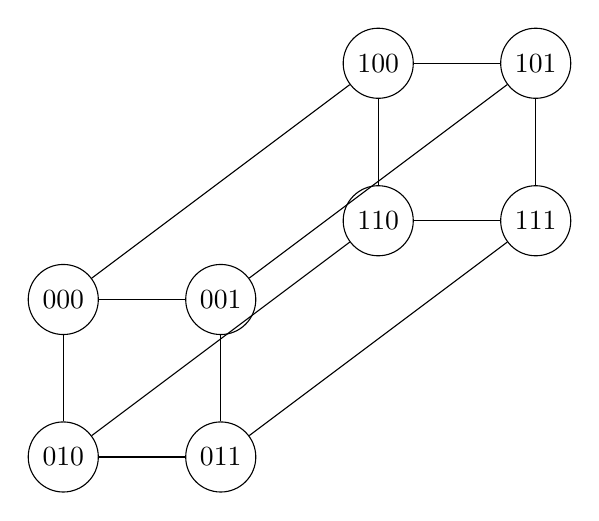
\begin{tikzpicture}
    \node[draw, circle] (000) at (0,0) {000};
    \node[draw, circle] (001) at (2,0) {001};
    \node[draw, circle] (011) at (2,-2) {011};
    \node[draw, circle] (010) at (0,-2) {010};
    \node[draw, circle] (110) at (4,1) {110};
    \node[draw, circle] (111) at (6,1) {111};
    \node[draw, circle] (101) at (6,3) {101};
    \node[draw, circle] (100) at (4,3) {100};

    \draw (000) -- (001) -- (011) -- (010) -- (000);
    \draw (100) -- (101) -- (111) -- (110) -- (100);
    \draw (000) -- (100);
    \draw (001) -- (101);
    \draw (011) -- (111);
    \draw (010) -- (110);
\end{tikzpicture}

$Q_{n+1}$ est construit à partir de $Q_n$ duppliqué.

On prend un cycle hamiltonien de $Q_n$. On enlève une arrête $(u,v)$ du cycle dans $Q_n$ :

$(u^0, v^0)$ dans $Q_{n+1}^0$ et $(u^1, v^1)$ dans $Q_{n+1}^1$.


\end{document}